\documentclass[12pt]{beamer}
\usetheme{UMNGolphers}
\usepackage{multicol}
\setlength{\columnsep}{0.5cm}



\title{\LARGE Limit Computation Using Asymptotic in CMS}
%\vskip400pt
\subtitle{\small UMN HEP Meeting}
\author{Tambe E. Norbert}
\date{\today}
%\institute{\url{norbert@physics.umn.edu}\\\url{http://www.physics.umn.edu/people/norbert.html}}
%\institute{ University of Minnesota,\\ \url{norbert@physics.umn.edu}}
\institute{ \url{norbert@physics.umn.edu}}


\begin{document}
% Align Titile in center
\begin{frame}[c]
\titlepage
\end{frame}
\section{Motivation}
\begin{frame}
\Large
\frametitle{Outline}
\tableofcontents
\end{frame}

\section*{Motivation}
\begin{frame}
\frametitle{Motivation}
%\vspace{-1cm}
\begin{itemize}
\Large{
\item <1-| alert@1> Quick computation of limits. 
%\item <1-| alert@1> Quick access to limits without need for resourceful Monte Carlo Computation.
\item  Study systematic effects.
%\item  Study the effects of uncertainties in a given measurement.
\item Extract experiment sensitivity without generating any Toy Monte Carlo.
%\item Easy approach to characterise the sensitivity of an experiment through the expected significance
\item  Quantify statistical significance of a signal.
%\item  Quantify statistical significance of an observed signal.
%\item Hypothesis Testing.
%\item Computing the confidence interval or upper limit of a given parameter
}
\end{itemize}
\begin{varblock}[7cm]{Data Compatibility?}
\[\label{eq:PVALUE}
 p-\mbox{value} = \left\lbrace 
  \begin{array}{ll}
  5.7 \times 10^{-7} , & \Rightarrow  \mbox{Reject Bkg-Only Hypo}\\
  < 0.05 ,& \Rightarrow  \mbox{Exclude Sig Hypo}
  \end{array}
 \right.
 \]
\end{varblock}
\end{frame}

\section{Statistical Formalism}
\begin{frame}
\frametitle{Statistical Test Formalism} 
\begin{minipage}{\textwidth}
Suppose a Poisson, $\mathcal{P}(n)$ of $n$ observed events with expected mean value $E[n] = \mu s + b$ 
 with systematics $\mathbf{\theta}$  then;
\end{minipage}\hfill

%\begin{multicols}{2}

\begin{minipage}{\textwidth}

 \begin{varblock}[7cm]{ProfileLikelihood and ratio}
  \begin{equation*}\label{eq:LL}
   \mathcal{L}(\mu, b,\theta) = \frac{(\mu s + b)^{n}}{n!}e^{-(\mu s + b)}\cdot \mathcal{L_{\theta}}(\theta) 
  \end{equation*}
  \begin{equation*}
   \lambda(\mu) = \frac{\mathcal{L}(\mu,\hat{\hat{\theta}})}{\mathcal{L}(\hat{\mu},\hat{\theta})} 
  \end{equation*}
 \end{varblock}
\end{minipage}
\begin{minipage}{\textwidth}
\begin{varblock}[7cm]{Test Statistics}
\[\label{eq:HNULL}
 t_{\mu} = \left\lbrace  
  \begin{array}{ll}
 -2\ln \lambda(\mu), & \hat{\mu} \leq \mu \\
   0,              & \hat{\mu} \geq \mu
  \end{array}
  \right.
\]
\end{varblock}
\end{minipage}
%\columnbreak
%\end{multicols}
\end{frame}


\section{Test Statistics Distribution}
\begin{frame}
\frametitle{Test Statistics Distribution}
\vspace{0.5cm}
 \begin{minipage}{\textwidth}
  Using the test statistics $t_{\mu}$,  We \alert{"find"} the pdf of the test statistics $f(t_{\mu}|\mu)$ assuming a given hypothesis $\mu$.
 \end{minipage}

%Finding significance involves Monte Carlo calculations $\Rightarrow$ computationally expensive.
%\begin{columns}[T] % align columns
%\begin{column}{.48\textwidth}
%\color{red}\rule{\linewidth}{4pt}

\begin{varblock}[7cm]{Asymptotic Method}
In Asymptotics, an analytic function of $f(t_{\mu}|\mu)$ through approximation(\alert{Walds}). 
\tiny{
\begin{equation*}
f(t_{\mu}|{\mu}^{\prime}) =\frac{1}{2\sqrt{t_{\mu}}}\frac{1}{\sqrt{2\pi}}\left[ \exp\left(-\frac{1}{2}(  \sqrt{t_{\mu}} + \frac{\mu - {\mu}^{\prime}}{\sigma})^{2}\right) +  \exp\left(-\frac{1}{2}(  \sqrt{t_{\mu}} - \frac{\mu - {\mu}^{\prime}}{\sigma})^{2}\right) \right]                            
\end{equation*}
}
%\mathbf{\Phi}\left(\frac{\mu -{\mu}^{\prime}}{\sigma}\right)\delta(t_{\mu})
\end{varblock}\hfill%
%\begin{column}{.48\textwidth}
%\color{blue}\rule{\linewidth}{4pt}
\vspace{-0.5cm}
%Right Part
\begin{varblock}[7cm]{HybridNew Method}
Through Monte Carlo or MCMC computations or toy experiments~(frequentest) one computes $f(t_{\mu}|\mu)$  after extracting $f(t_{\mu}|\mu)$ using Bayesian probability methods.
\end{varblock}\hfill
%\end{column}%
%\end{columns}
\end{frame}

\begin{frame}
\frametitle{Computing Probabilities}
\begin{minipage}{\textwidth}
Using $f(t_{\mu}|\mu)$, the probabilities~($p$-values) are computed as: 
%\vspace{-0.5cm}
  \begin{varblock}[7cm]{$p$-values}
    \begin{equation*}
     p_{u} = \int^{\infty}_{t_{\mu,obs}} f(t_{\mu}|\mu) dt_{\mu}
    \end{equation*}
   \end{varblock}
\end{minipage}

\begin{minipage}{\textwidth}
\vspace{0.5cm}
In the typical case where $\mu=1$ or $\mu=0$ for $s+b$ or $b$ only hypothesis $t =-2\ln(\frac{\mathcal{L}_{s+b}}{\mathcal{L}_{b}})$~(Tevatron style)
%\vspace{0.5cm}
  \begin{varblock}[7cm]{$CL_{s}$ Technique}
    \begin{equation*}
     CL_{s} = \frac{p_{s+b}}{1-p_{b}} = \frac{CL_{s+b}}{CL_{b}}
    \end{equation*}
   \end{varblock}
\end{minipage}
\end{frame}
%% Picture of Probability computation
\begin{frame}
\begin{figure}[ht]
%\begin{minipage}[b]{0.45\linewidth}
\centering
%\mbox{
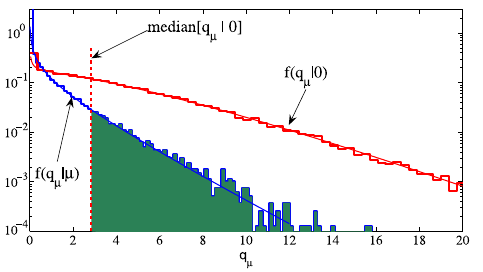
\includegraphics[height=5.5cm,width=5cm]{/home/tensr/Documents/TEN-HEP-PHD-THESIS/PHD_THESIS/PHD/THESISPLOTS/Test_Statistics_Asymptotic.png}
%}
%\caption{HYBRIDNEW}
\label{fig:Asymp}
%\end{minipage}
 \hspace{0.1cm}
% \begin{minipage}[b]{0.45\linewidth}
%\mbox{
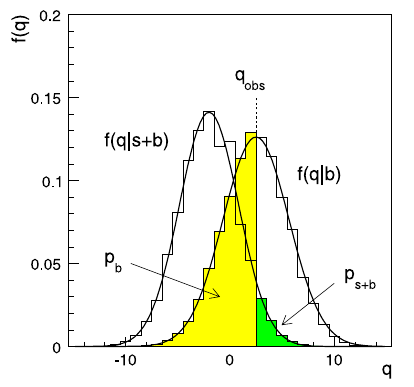
\includegraphics[height=5.5cm,width=5cm]{THESISPLOTS/TEST_STATISTICS.png}
%}
%\caption{>= 1 Jets Upper Limit $\chi^{0}_{1}$ Decay}
%\caption{ASYMTOTICS}
\label{fig:TeV}
% \end{minipage}
\end{figure}
\end{frame}





\section{Systematics}
\begin{frame}
\frametitle{Systematics}
%\vspace{-2cm}
\begin{varblock}[7cm]{Systematics in Asymptotic}
From the definition of $\mathcal{L}(\mu,b,\theta)$, systematics are introduced right on.
The approximate formula of the $f(t_{\mu}|\mu)$ analytically computed embeds in it systematics.
\end{varblock}
However, in HybridNew approach,
\begin{varblock}[7cm]{Systematics in HybridNew}
Integrate out systematics to get $f(t_{\mu}|\mu)$ .
\begin{equation*}
f(t) = \int f(t|\theta)\pi(\theta)d\theta
\end{equation*}
with $\pi(\theta) \propto \mathcal{L}_{\theta}(\theta)\pi_{0}(\theta)$ being the prior pdf.
\alert{This is how systematics are handled by the HybridNew approach}.
\end{varblock}
\end{frame}


\section{Application Example}
\begin{frame}
\frametitle{Application Example}
 \begin{varblock}[7.6cm]{Analysis Result}
  \begin{tabular}{c c}
   \hline
   \bfseries{SM Background/GMSB Signal} & \bfseries {Count}\\
   \hline \hline
   \texttt{Total SM background ($b$)} & $1.005 \pm 0.001$ \\
   \hline \hline
   \texttt{Data ($n_{obs}$)} & $1.00$ \\
   \hline \hline
   \texttt{Signal~($s$)}  &            \\
   \hline 
   \texttt{GMSB(SPS8)}~($\Lambda=180$~TeV,$c\tau=500$~mm) & $2.341$ \\
   \texttt{GMSB(SPS8)}~($\Lambda=180$~TeV,$c\tau=1000$~mm) & $4.585$ \\
   \texttt{GMSB(SPS8)}~($\Lambda=180$~TeV,$c\tau=2000$~mm) & $5.704$ \\
   \texttt{GMSB(SPS8)}~($\Lambda=180$~TeV,$c\tau=3000$~mm) & $5.386$ \\
   \texttt{GMSB(SPS8)}~($\Lambda=180$~TeV,$c\tau=6000$~mm) & $4.096$ \\ 
   \texttt{GMSB(SPS8)}~($\Lambda=180$~TeV,$c\tau=12000$~mm) & $2.772$ \\
   \hline
   \end{tabular}
 \end{varblock}
\end{frame}



\begin{frame}
\frametitle{Application Example}
 \begin{varblock}[7.5cm]{Sources of Systematics}
 % \begin{center}
  \begin{tabular}{c c}
  \hline
  \bfseries{Source} & \bfseries {Uncertainty(\%)}\\
  \hline
  \texttt{Photon energy scale}  & $< 3.0$\% \\
  \texttt{Jet energy scale}  & $< 0.05$\% \\
  \texttt{Jet energy resolution} &$ < 1.90$\% \\
  \texttt{PDF uncertainty} & $< 1.70$\% \\
  \texttt{MET resolution} & $ <2.8$\%  \\
  \texttt{Signal Eff $\times$ Acceptance}   &  $< 10$\% \\
  \texttt{ECAL time uncertainty} & $<5.0$\% \\
  \hline
  \texttt{Background estimation uncertainty} &$ \leq 20.0$\% \\
  \hline 
  \texttt{Luminosity}  & $< 2.2$\% \\
  \hline
  \end{tabular}
  %\captionof{table}{Summary of systematic uncertainties on the signal~(top), background~(middle) and machine~(bottom) as used in the $\sigma_{UL}$ calculation.}
  %\label{tab:SYST}
%\end{table}
 % \begin{center}
  \end{varblock}
 \end{frame}



\begin{frame}
\frametitle{Delayed Photon Upper Limit}
\begin{figure}[ht]
\begin{minipage}[b]{0.45\linewidth}
\centering
%\mbox{
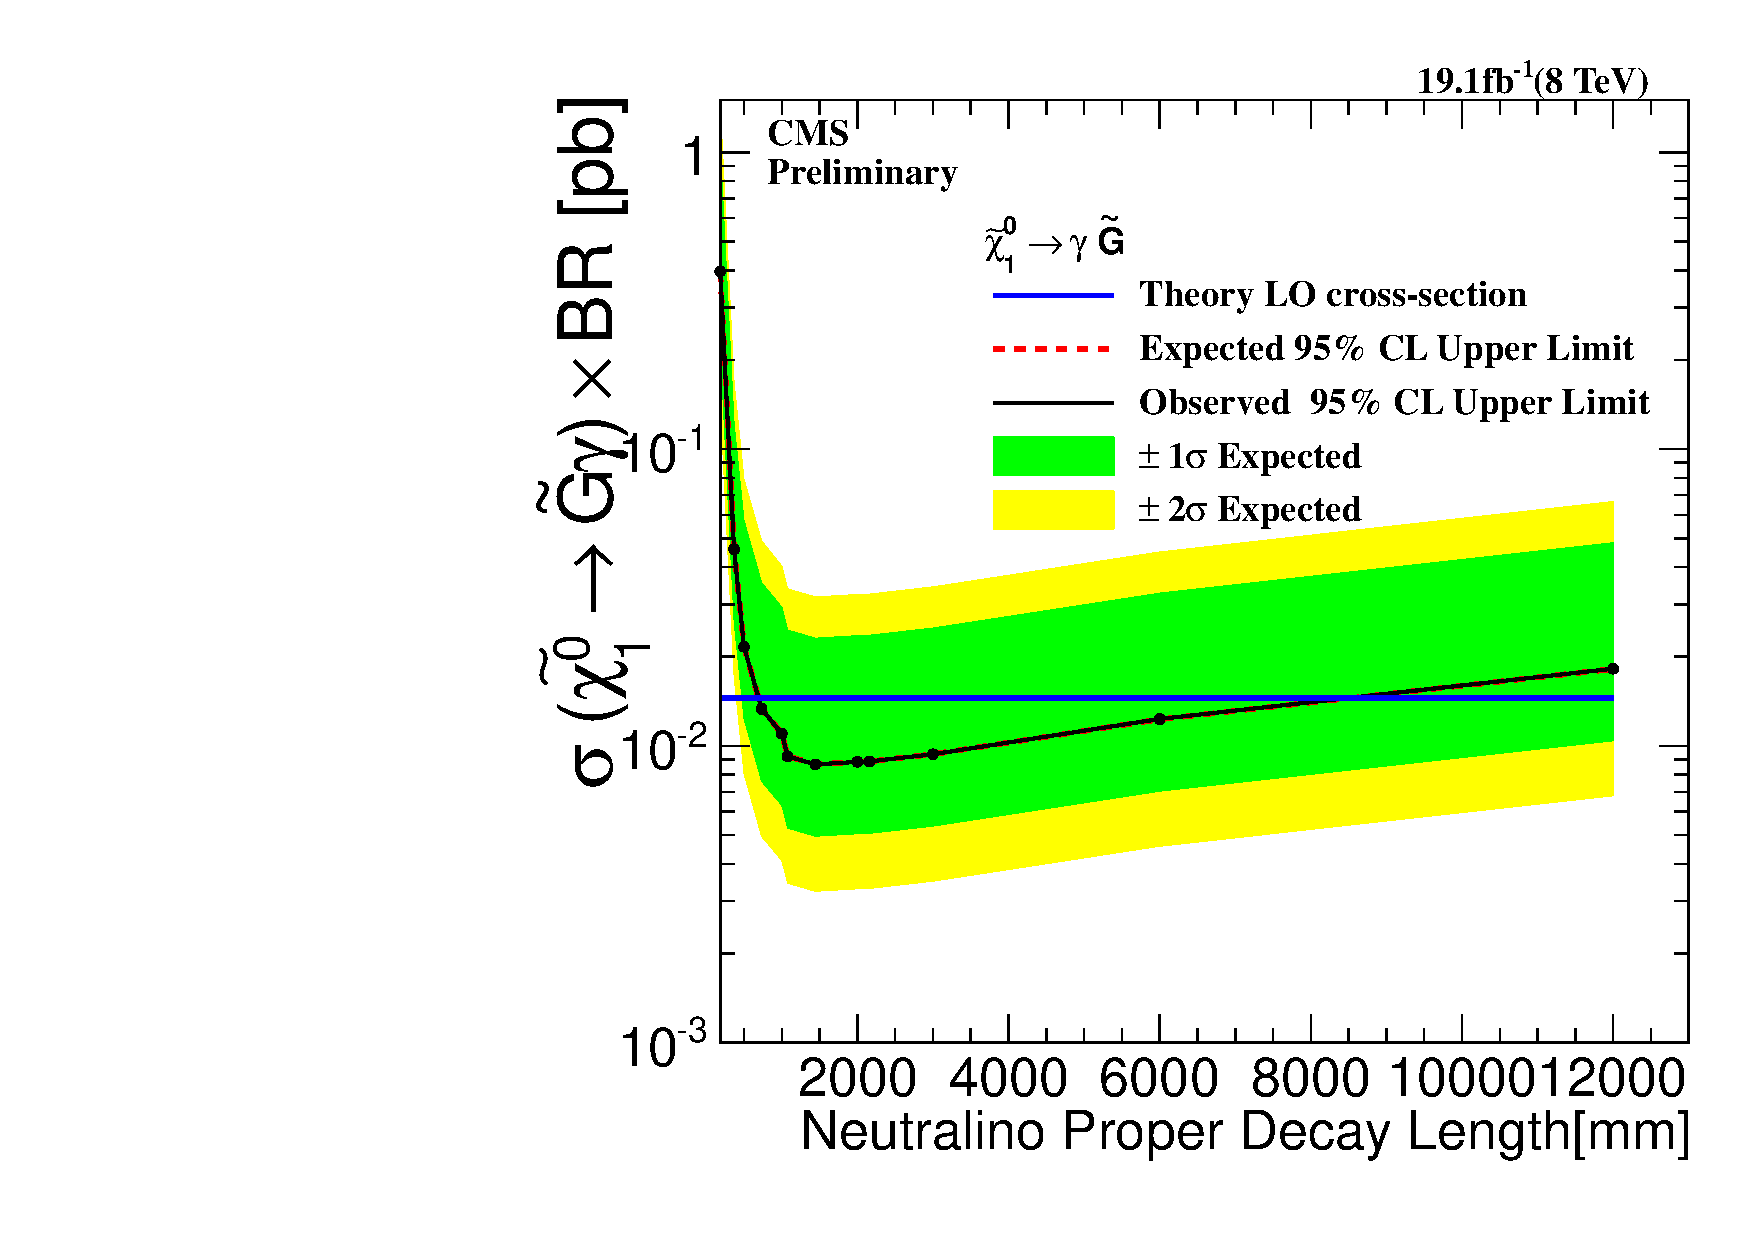
\includegraphics[height=5.5cm,width=5cm]{/home/tensr/Documents/TEN-HEP-PHD-THESIS/PHD_THESIS/PHD/THESISPLOTS/Asymptotics_wth_Systematics_Neutralino_CrossSecTimesBR_Uplimit.pdf}
%}
\caption{Systematics Inc.}
\label{fig:SUSY UL}
\end{minipage}
 \hspace{0.1cm}
 \begin{minipage}[b]{0.45\linewidth}
%\mbox{
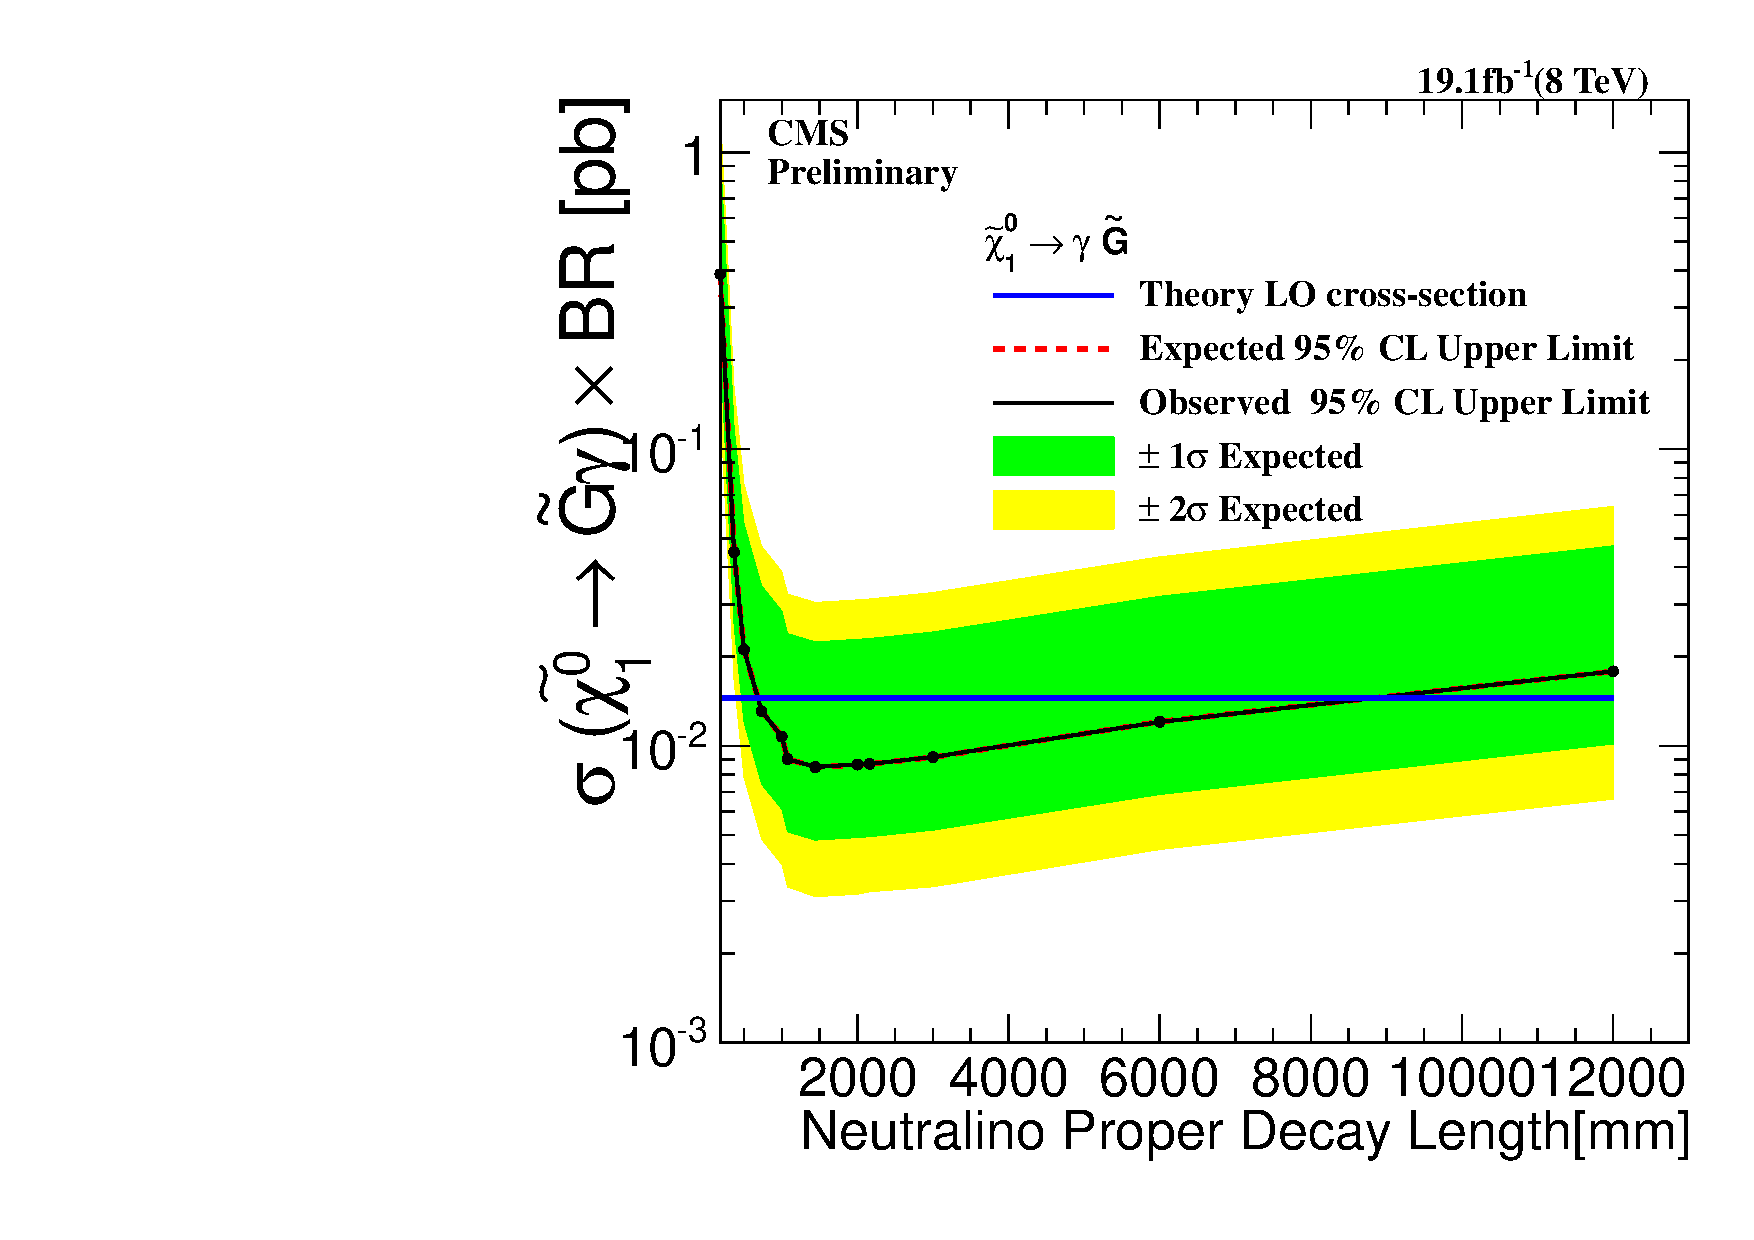
\includegraphics[height=5.5cm,width=5cm]{/home/tensr/Documents/TEN-HEP-PHD-THESIS/PHD_THESIS/PHD/THESISPLOTS/Asymtotics_Neutralino_CrossSecTimesBR_Uplimit.pdf}
%}
%\caption{>= 1 Jets Upper Limit $\chi^{0}_{1}$ Decay}
\caption{No Systematics}
\label{fig:SUSY UL}
 \end{minipage}
\end{figure}
\end{frame}

\begin{frame}
\frametitle{Extracting Upper Limits}
 \begin{varblock}[8cm]{Limits from P-values}
  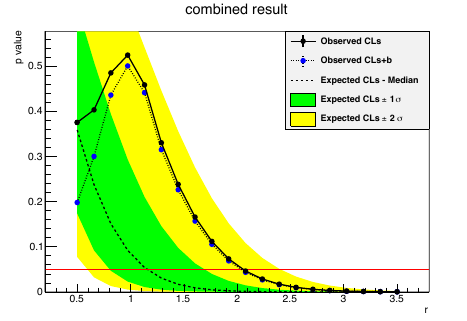
\includegraphics[scale=0.5]{/home/tensr/Documents/TEN-HEP-PHD-THESIS/PHD_THESIS/PHD/THESISPLOTS/Limits_CLs.png}
  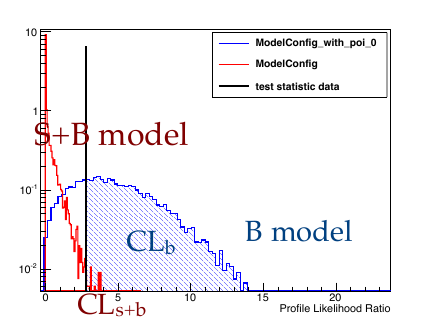
\includegraphics[scale=0.5]{/home/tensr/Documents/TEN-HEP-PHD-THESIS/PHD_THESIS/PHD/THESISPLOTS/Asymptotics_Test_Stats.png}
 \end{varblock}
\end{frame}

\begin{frame}
 %\begin{varblock}[8cm]{Test Statistics Distribution}
 \centering
  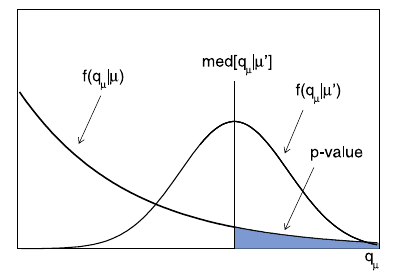
\includegraphics[scale=0.85]{/home/tensr/Documents/TEN-HEP-PHD-THESIS/PHD_THESIS/PHD/THESISPLOTS/Asymptotic_Generalised_Distribution_Of_Test_Statistics.png}
 %\caption{Asymptotic Te0.9ts Statistics}
% \end{varblock}
\end{frame}


% A bit about Asimov Dataset
\begin{frame}
\begin{varblock}[8cm]{"Asimov" Data"}
\frametitle{Asymptotic "Asimov" Dataset}
\begin{itemize}
\item Its an alternative way to obtain deviations from MLE~($\hat{\mu}$).
\item Is a Toy Monte Carlo data~(artificial data set),
\item Used to estimate the deviations; $\sigma$ from the median.
\item Also used to evaluate the value of $\hat{\mu}$ and $\hat{\theta}$
\item Obtaining the true parameters of the MLE.
\end{itemize}
\end{varblock}
\end{frame}


\begin{frame}
\frametitle{References}
\begin{itemize}
\item  Glen Cowan et al, \textit{Asymptotic formula for likelihood-based tests of new physics}, Eur.Phys.J.C~(2011)71:1554
\item A.L. Read, J.Phys. G $28$, 2693~(2002)
\item A. Wald. \textit{Tests of statistical hypothesis concerning several parameters when the number of observations is large.} Trans. Am. Maths. Soc 54(3), 426-482~(1943)
\item  Jose Ocariz \textit{Probability and Statistics for Particle Physicists}, arxiv:1405.3402v1
\item CERN Summer School: \tiny{https://indico.cern.ch/event/117033/material/slides/0?contribId=25}
\end{itemize}
\end{frame}

\end{document}